\section{Background Knowledge}
\label{sec:back}

Before starting our project, we first learned about what is function reactive programming and how is it different from object-oriented or imperative programming that we are familiar with.

We can understand the functional reactive programming by first divide it into two parts: Reactive Programming and Functional Programming.

\subsection{Reactive Programming}

Reactive Programming is a programming paradigm oriented around data flows and the propagation of change, i.e., asynchronous data streams. In our project, the data stream that we are handling is the network information, the questions and answers, and the feedbacks from the user.


\subsection{Functional Programming}

Functional programming is a style of programming which models computations as the evaluation of expressions. It concentrates on computing results rather than on performing actions.  Objects in a functional programming language are often immutable. 

Functional programming language usually have some nice features, including:

\begin{enumerate}
	\item Higher-order functions, i.e.,  functions that take other functions as their arguments. 
	\item Purity. Some functional languages can prohibit side effects like allowing expressions to yield actions in addition to return values. 
	\begin{enumerate}
		\item Purely functional programs typically operate on immutable data.
		\item Pure computations yield the same value each time they are invoked. This property is called referential transparency and makes possible to conduct equational reasoning on the code.
		\item Lazy evaluation
	\end{enumerate}
	\item Recursion. Recursion is heavily used in functional programming as it is the canonical and often the only way to iterate. 
\end{enumerate}


\subsection{Functional Reactive Programming}

Functional Reactive Programming integrates time flow and compositional events into functional programming. It provides an elegant way to express computation in domains such as interactive animations, robotics, computer vision, user interfaces, and simulation. In our project, we implemented an user interface to interactively visualize the data. The only thing that's mutable is the data flow, we don't want to change how the user interface looks like or how it will response to user actions.

\begin{figure}[h]
\centering
		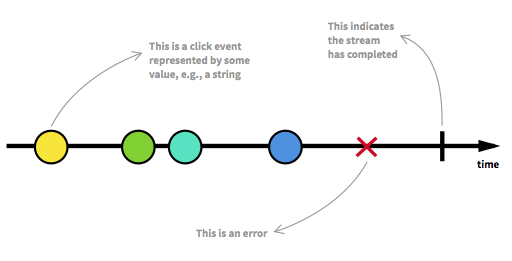
\includegraphics[width=\linewidth]{figure/frp_demo}
	\caption{Demonstration of data flow and compositional events}
	\label{fig:frp_demo}
\end{figure}




